% !TEX root = ../main.tex
% =============================================================================
% CHAPTER 4 - METHODOLOGY   (target ~16-18 pages)
% VOICE: impersonal passive. Never "we", never "I". See ../STYLE_GUIDE.md.
% Tense: SIMPLE PAST for procedures ("the signal was filtered", "the model was
% pretrained"); PRESENT for timeless model properties and equations ("the encoder
% consists of four blocks"; "let x denote..."). Be exact and reproducible. Put long
% hyperparameter tables in the Appendix and reference them.
% =============================================================================

\chapter{Methodology}\label{ch:method}

This chapter describes the methods used to develop, compare, and evaluate models
for resting-state EEG analysis. It is organised into seven sections covering the
datasets, EEG preprocessing, the proposed models, the comparison baselines,
self-supervised pretraining, downstream evaluation, and ablation studies and
model analysis.
Figure~\ref{fig:methodology_pipeline} provides an overview of the complete
methodological workflow.

% Generated by code/analysis/dataset/generate_method_figures.py, which writes the
% PDFs directly into manuscript/figures/. Authored at \textwidth (6.20 in) so the
% include applies no scaling. Do not resize here.
\begin{figure}[htbp]
\centering
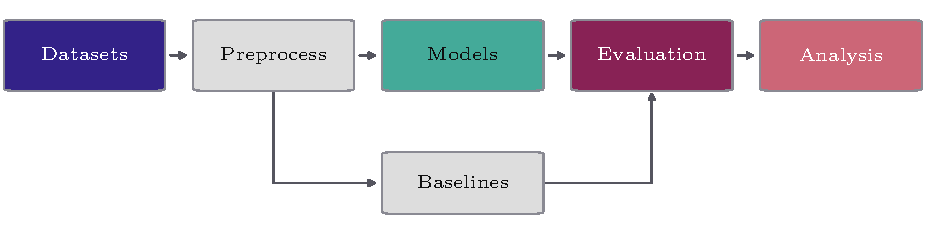
\includegraphics[width=\textwidth]{figures/fig_method_overview.pdf}
\caption[Overview of the methodological workflow]{Overview of the methodological
pipeline: a single preprocessing stage feeds both the self-supervised models and
the comparison baselines, which are then assessed under identical evaluation
protocols.}
\label{fig:methodology_pipeline}
\end{figure}


\section{Datasets}\label{sec:m_datasets}

Seven publicly available resting-state EEG datasets were included in this
study. Resting-state EEG is recorded while participants are not engaged in an
explicit cognitive task, typically under eyes-open or eyes-closed conditions.
The selected datasets differed in cohort composition, acquisition protocol,
electrode configuration, sampling rate, and recording duration. Including
datasets acquired from heterogeneous cohorts and under different recording
conditions was intended to reduce dependence on the characteristics of any
single dataset and to support the evaluation of cross-dataset generalisation.
The main characteristics of the seven datasets are summarised in
Table~\ref{tab:dataset_overview}.

% Generated by code/analysis/dataset/generate_table.py and copied here by
% code/analysis/sync_tables.py. Do not edit this file by hand.
\begin{table}[htbp]
  \centering
  \small
  \setlength{\tabcolsep}{5pt}
  \caption[Overview of the resting-state EEG datasets]{Acquisition characteristics of the seven resting-state EEG datasets.}
  \label{tab:dataset_overview}
  \resizebox{\ifdim\width>\linewidth\linewidth\else\width\fi}{!}{%
  \begin{tabular}{l l l l c c c c}
    \toprule
    \textbf{Dataset} & \textbf{Accession} & \textbf{Stage} & \textbf{Participant groups} & \textbf{Ch.} & \shortstack{\textbf{Frequency}\\\textbf{(Hz)}} & \textbf{Cond.} & \textbf{Dur.\ (min)} \\
    \midrule
    DVS & ds005385 & Pretraining & 542 HC & 64 & 1000 & EO, EC & 3.1 \\
    SRM & ds003775 & Pretraining & 111 HC & 64 & 1024 & EC & 4.0 \\
    LEMON & -- & Pretraining & 215 HC & 61 & 2500 & EO & 17.4 \\
    ADFTD & ds004504 & Downstream & 36 AD, 23 FTD, 29 HC & 19 & 500 & EC & 13.4 \\
    FEP & ds003944 & Downstream & 47 FEP, 30 HC & 61 & 1000 & EO & 5.1 \\
    MDD & ds003478 & Downstream & 32 MDD, 90 HC & 64 & 500 & EO, EC & 5.8 \\
    SCZ & -- & External test & 30 SCZ, 47 HC & 64 & 1000 & EC & 2.2 \\
    \bottomrule
  \end{tabular}%
  }
  \\[3pt]
  \begin{minipage}{\linewidth}\footnotesize\raggedright
    Participant groups are the participants retained after preprocessing, before the pretraining-reserve split (Figure~\ref{fig:dataset_partitioning}). Ch.: EEG channels. Cond.: recording condition, eyes open (EO) or eyes closed (EC). Dur.: mean recording length. HC: healthy control. AD: Alzheimer's disease. FTD: frontotemporal dementia. FEP: first-episode psychosis. MDD: major depressive disorder. SCZ: schizophrenia.
  \end{minipage}
\end{table}


Three datasets comprised healthy control participants only: the Dortmund Vital
Study \parencite[DVS;][]{edmundwascherRestingstateEEGData2025}, the SRM dataset
\parencite{christofferhatlestad-hallSRMRestingstateEEG2022}, and the Leipzig
Study for Mind-Body-Emotion Interactions
\parencite[LEMON;][]{babayanMindbrainbodyDatasetMRI2019}. The remaining four
datasets included both participants with a clinical diagnosis and healthy
controls: the Alzheimer's disease and frontotemporal dementia dataset
\parencite[ADFTD;][]{miltiadousDatasetScalpEEG2023a}, the first-episode
psychosis dataset \parencite[FEP;][]{deansalisburyEEGFirstEpisode2022}, the
major depressive disorder dataset \parencite[MDD;][]{ds003478:1.1.0}, and the
schizophrenia dataset \parencite[SCZ;][]{raczReducedTemporalVariability2025}.

The datasets were allocated across three stages of the study:
self-supervised pretraining, downstream clinical evaluation, and external
testing. An overview of the dataset and participant allocation is provided in
Figure~\ref{fig:dataset_partitioning}.

% The four figures below are generated by code/analysis/dataset/generate_figures.py,
% which writes the PDFs directly into manuscript/figures/. Each is authored at
% \textwidth (6.20 in) so the includes apply no scaling. Do not resize them here.
\begin{figure}[htbp]
\centering
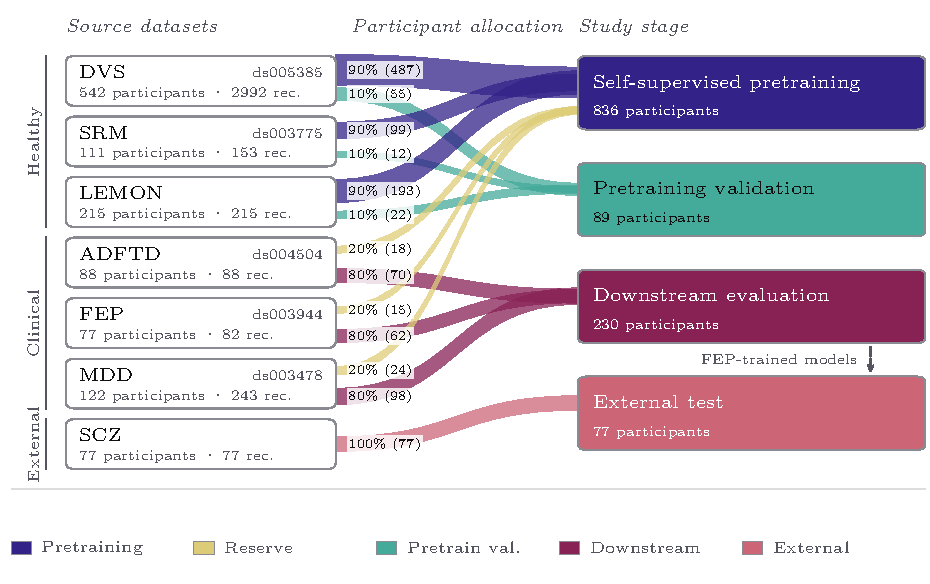
\includegraphics[width=\textwidth]{figures/fig_dataset_allocation.pdf}
\caption[Allocation of datasets to study stages]{Allocation of the seven
resting-state datasets and their participants to the stages of the study;
partitions are defined at the participant level, so no participant contributes to
both pretraining and downstream evaluation.}
\label{fig:dataset_partitioning}
\end{figure}

DVS, SRM, and LEMON formed the primary self-supervised pretraining corpus.
These datasets were selected to expose the model to resting-state EEG
recordings obtained from multiple cohorts and acquisition settings. This
selection was intended to reduce the likelihood that the model would learn
representations specific to a single dataset. Within each dataset, 90\% of the
participants were allocated to the training set during self-supervised pretraining, while the remaining
10\% formed a held-out validation set. The validation participants were used
exclusively to monitor model performance during pretraining.

ADFTD, FEP, and MDD were used primarily for downstream clinical evaluation.
However, restricting self-supervised pretraining to healthy control datasets
would have limited the participant level and neurophysiological variability
represented in the pretraining corpus. Therefore, 20\% of participants from
each of these datasets were allocated to a separate pretraining reserve
subset. Each reserve subset included participants from both the clinical and
healthy control groups. These subsets were added to the self-supervised
pretraining corpus to broaden the range of resting-state EEG characteristics
represented during pretraining. The remaining 80\% of participants in each
dataset formed the downstream evaluation pool.

The resulting pretraining corpus and its demographic composition are shown in
Figure~\ref{fig:pretrain_cohorts}.

All dataset partitions were defined at the participant level to prevent data
leakage between study stages. Participants assigned to the
pretraining reserve subsets were used exclusively for self-supervised
pretraining and were excluded from all downstream analyses. Consequently, no
participant contributed data to both pretraining and downstream performance
evaluation. This separation maintained participant level independence between
the two stages.

The SCZ dataset was excluded from both self-supervised pretraining and
in-domain downstream model development. Instead, it was used exclusively as an
external test set for models developed using the FEP dataset. Differences between the FEP and SCZ datasets in cohort composition and
acquisition conditions introduced a distribution shift between the development
and external test data. This design was intended to provide a more stringent
assessment of cross-dataset generalisation.

The composition of the four downstream cohorts and of the external test set,
including their age and sex distributions, is shown in
Figure~\ref{fig:downstream_cohorts}. The cohorts differ substantially in age:
the dementia cohorts are elderly, whereas the FEP and MDD cohorts are drawn from
young adults. The proportion of patients also varies across cohorts, which
determines the chance level of the metric reported in
Section~\ref{sec:m_protocols}.

\begin{figure}[htbp]
\centering
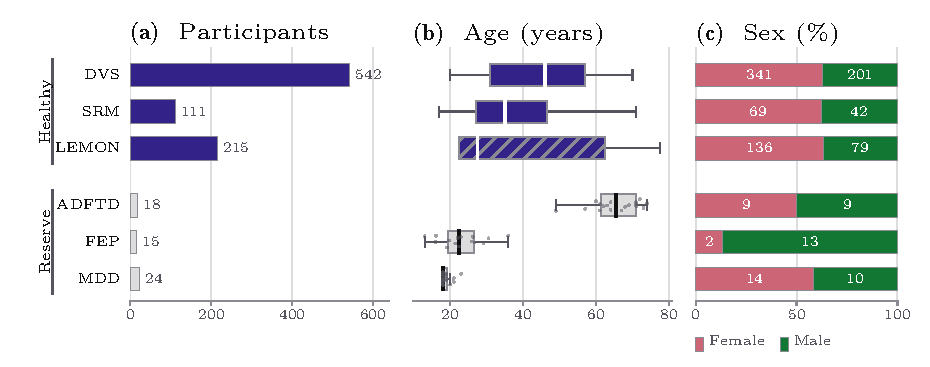
\includegraphics[width=\textwidth]{figures/fig_pretrain_cohorts.pdf}
\caption[Composition of the pretraining corpus]{Composition of the
self-supervised pretraining corpus by source dataset: participants (a), age (b),
sex (c). LEMON's age (hatched) is approximate, built from published five-year
brackets.}
\label{fig:pretrain_cohorts}
\end{figure}

\begin{figure}[htbp]
\centering
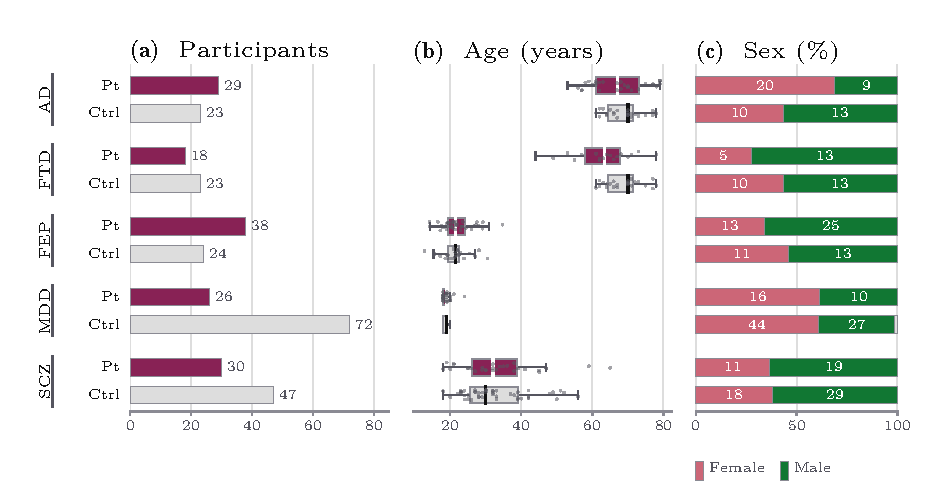
\includegraphics[width=\textwidth]{figures/fig_downstream_cohorts.pdf}
\caption[Composition of the downstream cohorts]{Composition of the four downstream evaluation cohorts and external SCZ test set: participants (a), age (b), and sex (c). Pt/Ctrl: patients/controls. AD and FTD share controls from the same 70-participant ADFTD pool. One MDD control had unrecorded age and sex, resulting in one fewer count in (b) and (c).
}
\label{fig:downstream_cohorts}
\end{figure}


\section{Preprocessing}\label{sec:m_preprocess}

% TODO: The exact chain, in order: read EEGLAB .set -> pick EEG channels -> V->uV
% scaling -> EEGPrep (DC offset, resample to 200 Hz, flatline & drift removal,
% RANSAC bad channel detection, ASR burst removal, bad window rejection, average
% re-reference) -> bandpass 0.5-45 Hz -> 50 Hz notch -> ICA + ICLabel artefact
% rejection -> fixed-length windowing (15 s / 3000 samples, non-overlapping).
% Channel standardisation: strict global channel-name intersection (19 common
% channels, no padding); per-window per-channel z-score normalisation. Justify
% non-overlapping windows (avoids train/eval leakage; LaBraM standard).



EEG preprocessing was performed to reduce technical noise and physiological artefacts while preserving neural activity relevant to the subsequent analyses. Scalp-recorded EEG does not provide a noise-free representation of brain activity, as recordings may contain slow signal drift, power-line interference, malfunctioning electrodes, and artefacts caused by eye movements, cardiac activity, and muscle contractions. These sources can obscure the underlying neural signals and reduce the reliability of subsequent analyses. Because the seven datasets were collected using different acquisition systems and sampling frequencies, the same general preprocessing pipeline was applied to all datasets to improve signal comparability and produce consistently structured inputs. The complete ordered pipeline is shown in Figure~\ref{fig:preprocessing_pipeline}.

\begin{figure}[htbp]
\centering
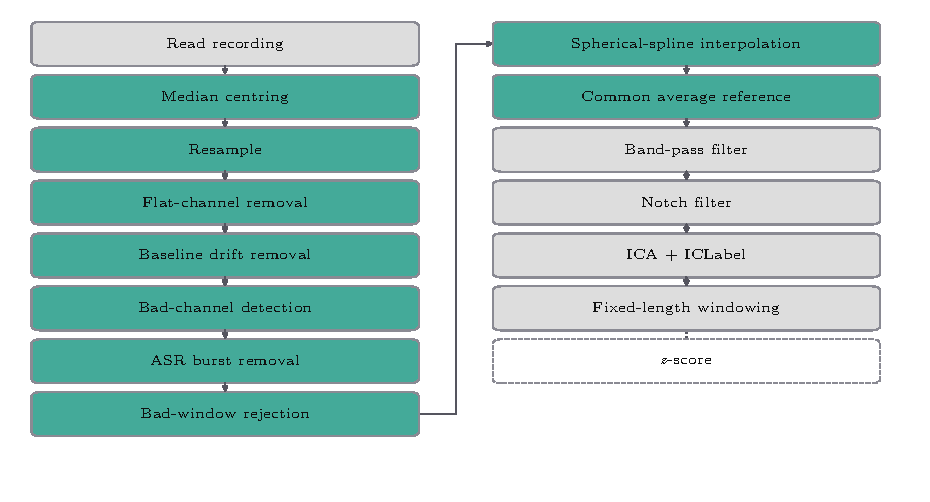
\includegraphics[width=\textwidth]{figures/fig_preprocessing_pipeline.pdf}
\caption[The preprocessing pipeline]{The preprocessing pipeline, shown in the order of application. Tinted stages are performed by the EEGPrep pipeline.}
\label{fig:preprocessing_pipeline}
\end{figure}

Each recording was loaded using the \texttt{MNE-Python} library \parencite{gramfortMEGEEGData2013}. Only channels identified as EEG channels were retained, while non-EEG channels, including stimulation and auxiliary channels, were excluded. \texttt{MNE-Python} internally represents EEG amplitudes in volts; therefore, the signals were converted to microvolts by multiplying them by \(10^{6}\). This operation changed only the unit of measurement and made the signal amplitudes easier to interpret and use during subsequent processing.

The recordings were then processed using the EEGPrep pipeline provided by the \texttt{Braindecode} library \parencite{7274673,aristimunhaBraindecodeToolboxDecoding2026}. EEGPrep applies a standardised sequence of procedures that includes offset correction, resampling, flat channel removal, drift attenuation, bad channel detection, transient artefact correction, bad window rejection, channel interpolation, and re-referencing. Applying the same ordered procedure to all datasets reduced variability arising from dataset specific preprocessing choices.

First, the channel-wise DC offset was removed by subtracting the temporal median of each channel:

\begin{equation}
X'_{c,t}
=
X_{c,t}
-
\underset{\tau}{\operatorname{median}}
\left(X_{c,\tau}\right)
\label{eq:median_centering}
\end{equation}

where \(c\) denotes the EEG channel, \(t\) denotes the current time sample, and \(\tau\) indexes the time samples used to calculate the channel median. Throughout this section, \(X\) denotes the signal at the input of the operation being described and \(X'\) the signal it produces. Median centring removes constant channel offsets while being less sensitive than mean subtraction to isolated high-amplitude values.

The datasets were originally recorded at different sampling frequencies. All recordings were therefore resampled to a common sampling frequency of \(200\)~Hz. Standardising the sampling frequency ensured that signals of equal duration contained the same number of samples across datasets and reduced the computational and storage requirements of the subsequent analyses. At \(200\)~Hz, the Nyquist frequency is \(100\)~Hz, which is substantially higher than the final upper passband frequency of \(45\)~Hz. The resampling procedure thus retained the complete frequency range examined in this study.

Channels that remained flat for more than \(5\)~s were identified as unusable and temporarily removed. Flat channels contain little or no electrophysiological information and may adversely affect spatial interpolation and common-average re-referencing. EEGPrep also applied its default drift removal high-pass transition band of \(0.25\)-\(0.75\)~Hz before identifying additional unreliable channels.

Additional bad channels were detected using correlation-based procedures derived from the PREP framework \parencite{bigdely-shamloPREPPipelineStandardized2015a}. The signal recorded at each channel was compared with a spatial prediction derived from the remaining channels. Channels with a correlation below \(0.75\) were classified as unreliable. High-frequency noise measures were also used to identify electrodes dominated by non-physiological noise, even when the channels were not completely flat. The correlation threshold of \(0.75\) provided a relatively permissive criterion that reduced the likelihood of rejecting channels that retained usable information.

Transient high-amplitude artefacts were subsequently corrected using Artifact Subspace Reconstruction (ASR). ASR compares short-term multichannel activity with a reference distribution obtained from relatively clean portions of the recording. Signal subspaces exhibiting abnormally high variance are identified and reconstructed using the retained subspaces of the calibration model. An ASR burst removal cutoff of \(20\) was used. Because higher cutoff values result in less aggressive correction, this value provided a conservative balance between suppressing large transient artefacts and preserving potentially meaningful neural activity.

After ASR, EEGPrep removed time intervals containing widespread residual contamination. A time interval was classified as unreliable when more than \(25\%\) of its channels exceeded the permitted amplitude tolerance. The default upper tolerance of seven standard deviations was used, with no finite lower threshold. 

% For the selection of ASR calibration data, a stricter maximum proportion of $7.5\%$ bad channels and an upper tolerance of $5.5$ standard deviations were used.

Channels previously identified as flat or unreliable were then reconstructed using spherical-spline interpolation based on the spatial distribution of the retained electrodes. Reinterpolation restored the expected channel configuration and prevented the number of input channels from varying according to the channels rejected in individual recordings.

The signals were subsequently re-referenced using a common average reference. At each time point, the mean amplitude across all retained and reconstructed EEG channels was subtracted from the amplitude of each channel:

\begin{equation}
X'_{c,t}
=
X_{c,t}
-
\frac{1}{C}
\sum_{i=1}^{C} X_{i,t}
\label{eq:common_average_reference}
\end{equation}

where \(C\) denotes the total number of EEG channels included in the reference, \(c\) denotes the channel being re-referenced, and \(i\) is the summation index. Re-referencing was performed after bad channel correction to prevent severely contaminated channels from disproportionately influencing the average reference. The common average reference also provided a consistent reference convention across datasets that may originally have been recorded using different physical references. However, its effectiveness depends on the number and spatial coverage of the available electrodes.

Following EEGPrep, the recordings were band-pass filtered between \(0.5\) and \(45\)~Hz using the default zero-phase finite impulse response filtering procedure provided by \texttt{MNE-Python}. The lower cutoff attenuated slow baseline drift, while the upper cutoff reduced high-frequency instrumental and muscular noise. Activity outside this frequency range was excluded from the present analysis rather than assumed to be entirely non-neural.

A notch filter was then applied at the local electrical mains frequency. A frequency of \(50\)~Hz was used for the European datasets, while \(60\)~Hz was used for the datasets recorded in the United States. The notch filter was applied as a fixed component of the standardised preprocessing pipeline. Because the preceding \(45\)~Hz low-pass filter already attenuated activity at \(50\) and \(60\)~Hz, the notch filter was expected to provide only limited additional suppression of power-line interference. It was nevertheless retained to maintain a uniform procedure across datasets.

Independent component analysis \parencite[ICA;][]{hyvarinenIndependentComponentAnalysis2000} was subsequently used to reduce structured physiological and non-neural artefacts that remained after the preceding cleaning operations. For each recording, a separate copy of the signal was high-pass filtered at \(1\)~Hz. FastICA was then fitted to this copy using a maximum of \(20\) independent components. For recordings containing fewer channels, the number of components was limited to one fewer than the number of available EEG channels. A fixed random seed of \(42\) was used to improve the reproducibility of the decomposition. Fitting ICA on a \(1\)~Hz high-pass-filtered copy reduced the influence of slow signal fluctuations and improved the stability of the decomposition.

The resulting independent components were automatically classified using ICLabel through the \texttt{MNE-ICALabel} library \parencite{Li2022}. ICLabel estimates the probability that each component represents brain activity, muscle artefact, ocular artefact, cardiac activity, line noise, channel noise, or other activity. A component was excluded when its predicted class was muscle artefact, eye blink artefact, cardiac activity, line noise, or channel noise and the corresponding classification probability was at least \(0.80\). This relatively high threshold was used as a conservative criterion so that components were removed only when the classifier expressed strong confidence that they were artefactual.

The ICA solution estimated from the \(1\)~Hz high-pass-filtered copy was then applied to the corresponding \(0.5\)-\(45\)~Hz signal. This procedure allowed the decomposition to be estimated from data with reduced slow drift while preserving the lower-frequency activity included in the final analysis.

The effect of the complete pipeline on a single recording is shown in
Figure~\ref{fig:preprocessing_effect}, together with the independent components
that ICLabel classified for that recording.

% Panels (a)-(d) are built from outputs/cache/preprocessing_example.npz, which
% code/analysis/dataset/extract_preprocessing_example.py writes by running the
% real pipeline on one recording. That script has to run where the EEG data
% lives; the figure builder in generate_method_figures.py only reads the cache.
\begin{figure}[p]
\centering
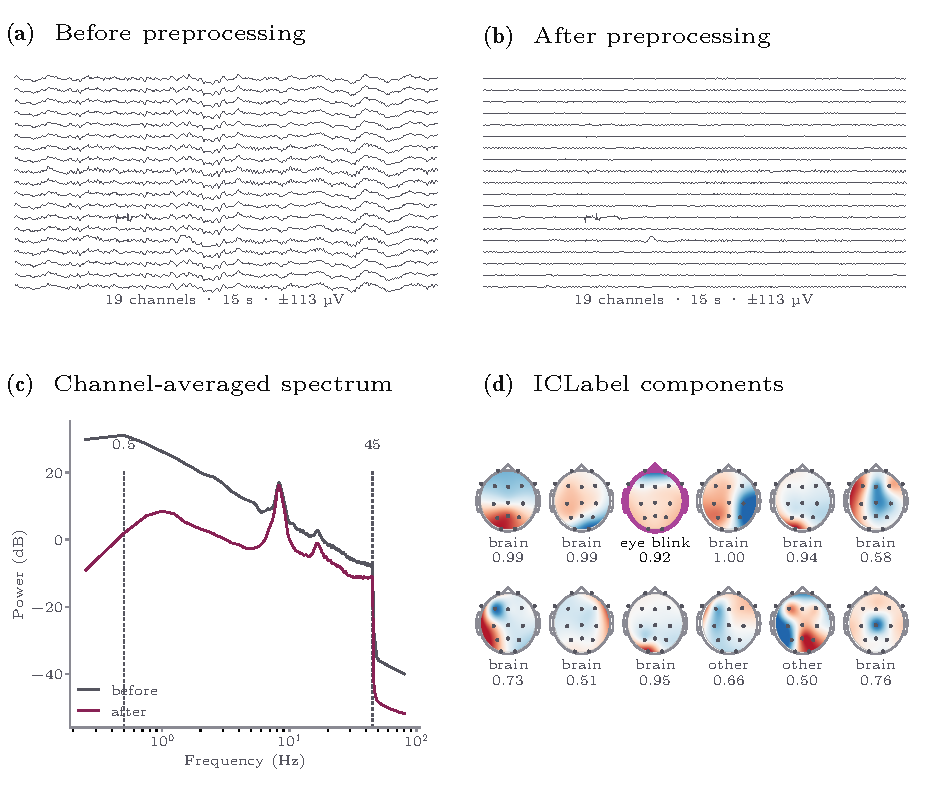
\includegraphics[width=\textwidth]{figures/fig_preprocessing_effect.pdf}
\caption[The preprocessing pipeline applied to one recording]{Preprocessing pipeline applied to a healthy subject (sub-037) from ADFTD dataset. \textbf{(a,b)} The same 15-s excerpt before and after preprocessing, shown at a shared amplitude scale defined by the 99.5th percentile of the raw signal amplitude, so that the removal of slow drift and large transients is directly visible. \textbf{(c)} Channel-averaged power spectral density before and after preprocessing, with the passband edges marked. \textbf{(d)} Independent components with their ICLabel class and probability; outlined components were removed based on an artefact-class probability of \(\geq 0.80\).}
\label{fig:preprocessing_effect}
\end{figure}

One limitation of this procedure is that ICLabel was originally developed using extended-Infomax ICA decompositions, whereas the present pipeline used FastICA. The data otherwise followed the principal ICLabel preprocessing recommendations because they were common-average referenced and ICA was fitted using a \(1\)~Hz high-pass-filtered copy. Nevertheless, the difference in ICA algorithm may affect the reliability of the automatic component classifications and should be considered when interpreting the results.

Following artefact removal, each recording was divided into fixed-length, non-overlapping windows of \(15\)~s. At a sampling frequency of \(200\)~Hz, each window contained \(3000\) time samples. A fixed window duration ensured that all inputs had identical temporal dimensions. The \(15\)~s duration provided a compromise between temporal resolution, computational requirements, the number of available windows, and the amount of temporal context represented within each window. In particular, a \(15\)~s window contains approximately \(7.5\) cycles of activity at the lower passband frequency of \(0.5\)~Hz.

Non-overlapping windows were used to avoid generating highly similar samples containing duplicated time points. Any incomplete window containing fewer than \(3000\) samples at the end of a recording was discarded.

Z-score normalisation was not applied as part of the preprocessing pipeline described above and was not stored in the saved EEG windows. Instead, it was performed when the data were loaded for the supervised deep learning and self-supervised learning models. Each channel within each \(15\)~s window was normalised independently using the temporal mean and standard deviation calculated from that channel within the same window:

\begin{equation}
\widetilde{X}_{w,c,t}
=
\frac{
X_{w,c,t} - \mu_{w,c}
}{
\sigma_{w,c} + \varepsilon
}
\label{eq:window_zscore}
\end{equation}

where \(w\) denotes the window, \(c\) denotes the EEG channel, \(t\) denotes the time sample, and \(\varepsilon\) is a small positive constant included to prevent division by zero. The within-window temporal mean was calculated as

\begin{equation}
\mu_{w,c}
=
\frac{1}{T}
\sum_{\tau=1}^{T} X_{w,c,\tau}
\label{eq:window_channel_mean}
\end{equation}

and the corresponding standard deviation was calculated as

\begin{equation}
\sigma_{w,c}
=
\sqrt{
\frac{1}{T}
\sum_{\tau=1}^{T}
\left(
X_{w,c,\tau} - \mu_{w,c}
\right)^{2}
}
\label{eq:window_channel_std}
\end{equation}

where \(T=3000\) denotes the number of time samples in each window and \(\tau\) is the summation index over those samples. Because the mean and standard deviation were calculated independently for each channel and window, no normalisation statistics were shared across participants or between the training, validation, and test partitions. This procedure therefore did not introduce information leakage between the data partitions.

The traditional machine learning models followed a different normalisation procedure. The EEG windows used for these models were not z-score normalised during data loading. Instead, the extracted feature vectors were standardised using a standard scaler fitted exclusively to the training fold and subsequently applied to the corresponding validation and test folds. This ensured that the traditional machine learning analyses also avoided information leakage.


% Two full-page floats live in the preprocessing section; flush them before
% the next section starts so they do not drift into it.
\FloatBarrier

\section{Proposed Models}\label{sec:m_models}

This study developed three self-supervised models for learning representations from resting-state EEG: BrainLM-EEG, BrainLM-EEG-RoPE, and BrainLM-EEG-Microstate. BrainLM \parencite{caroFOUNDATIONMODELBRAIN2024a} was originally introduced as a foundation model for fMRI and uses masked autoencoding \parencite{heMaskedAutoencodersAre2022} to learn spatiotemporal representations from brain activity. Here, the BrainLM framework was adapted to EEG, resulting in BrainLM-EEG, which serves as the reference architecture for the two subsequent extensions.

Adapting BrainLM to EEG required reformulating its spatiotemporal input representation around EEG electrodes and short temporal signal patches. BrainLM-EEG retains the core masked encoder-decoder learning principle while representing each EEG window as a sequence of channel-specific temporal patches. Building on this architecture, BrainLM-EEG-RoPE replaces learned spatial channel embeddings with geometry-aware rotary positional encoding derived from electrode locations, while BrainLM-EEG-Microstate augments the masked reconstruction objective with an auxiliary prediction task based on canonical EEG microstates.

Each extension modifies a single aspect of BrainLM-EEG while retaining the same input representation, Transformer backbone, masking strategy, and pretraining data. This controlled design enables the effect of each modification to be evaluated separately.

The proposed models were compared with three groups of established methods, described in Section~\ref{sec:m_baselines}.


\subsection{BrainLM-EEG: Adapting BrainLM to EEG}\label{sec:m_brainlmeeg}

BrainLM-EEG adapted the masked autoencoding framework of BrainLM from fMRI to
resting-state EEG. The original BrainLM represents fMRI as spatiotemporal
patches defined over brain parcels and time. In BrainLM-EEG, the corresponding
spatial units are EEG electrodes, and each electrode signal is divided into
short temporal patches. The model is pretrained by reconstructing randomly
masked channel-time patches from the remaining visible EEG context. Unless
stated otherwise, the architectural and training choices described in this
subsection were shared by BrainLM-EEG, BrainLM-EEG-RoPE, and
BrainLM-EEG-Microstate.

\medskip\noindent\textbf{Input representation and tokenisation}\par
Following preprocessing, each EEG recording was segmented into non-overlapping
15-second windows. Because the included datasets differed in electrode
configuration, the analysis was restricted to a common set of 19 channels
corresponding to the standard international 10-20 montage. The electrodes and
the order in which the model received them are listed in
Appendix~\ref{app:montage}. All
signals were resampled to 200~Hz. Each input window was therefore represented as

\begin{equation}
    \mX \in \sR^{C \times T},
    \qquad C = 19,
    \qquad T = 3000
    \label{eq:brainlmeeg_input}
\end{equation}

where \(C\) denotes the number of channels and \(T\) denotes the number of time
points.

Each channel was divided into 15 non-overlapping temporal patches of one
second, with 200 time points per patch. A 15-second window consequently
produced

\begin{equation}
    N = C \times P = 19 \times 15 = 285
    \label{eq:brainlmeeg_tokens}
\end{equation}

spatiotemporal tokens, where \(P=15\) denotes the number of temporal patches
per channel. Each token represented one electrode during a specific one-second
interval. A linear projection mapped each 200-sample patch to a
512-dimensional embedding. The construction of the token sequence is shown in
Figure~\ref{fig:architecture_overview}.

% \begin{figure}[htbp]
% \centering
% 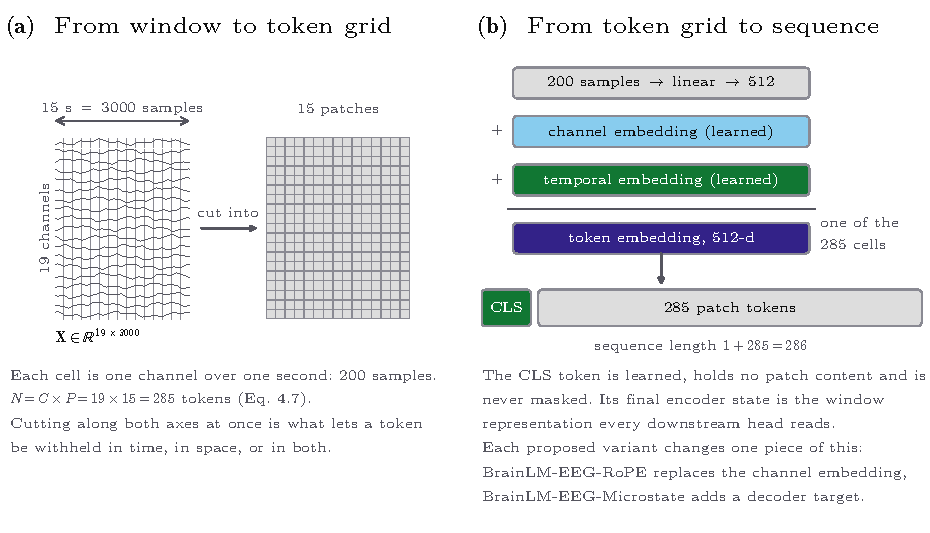
\includegraphics[width=\textwidth]{figures/fig_tokenisation.pdf}
% \caption[From a 15-second window to the encoder sequence]{Construction of the
% input sequence. \textbf{(a)}~Each \(15\)~s window is cut along both the channel
% and the time axis into one-second patches, giving the \(19 \times 15\) grid of
% spatiotemporal tokens on which the masking strategies of
% Figure~\ref{fig:masking_schemes} operate. \textbf{(b)}~Each patch is projected to
% 512 dimensions and summed with a learned channel embedding and a learned temporal
% embedding; a learned CLS token is prepended, giving a sequence of length
% \(286\). Each proposed variant modifies exactly one element of this construction:
% BrainLM-EEG-RoPE replaces the channel embedding
% (Section~\ref{sec:m_rope}), and BrainLM-EEG-Microstate adds a second decoder
% target (Section~\ref{sec:m_microstate}).}
% \label{fig:tokenisation}
% \end{figure}

\medskip\noindent\textbf{Positional representation and sequence construction}\par
The reference BrainLM-EEG model used separate learnable embeddings for spatial
and temporal position. For each token, the patch embedding was combined with a
channel embedding identifying the corresponding electrode and a temporal
embedding identifying its position within the 15-second window.

A learnable classification token, denoted CLS, was prepended to the
token sequence. The CLS token had the same 512-dimensional embedding
size as the patch tokens and was intended to aggregate information across the
complete input window. Its final encoder representation was used as the global
representation for downstream classification.

\medskip\noindent\textbf{Encoder-decoder architecture}\par
The encoder comprised four transformer blocks with an embedding dimension of
512 and four self-attention heads. The dimension of each attention head was
therefore 128. Within each block, the feed-forward network expanded the
representation dimension by a factor of four before projecting it back to 512
dimensions. Gaussian error linear unit
\parencite[GELU;][]{hendrycksGaussianErrorLinear2023} activations were used in
the feed-forward layers.

The decoder comprised two transformer blocks with the same embedding dimension
and number of attention heads. It was deliberately shallower than the encoder
so that the encoder was required to learn informative latent representations
that supported reconstruction using a comparatively lightweight decoder. A
linear reconstruction head mapped each decoder output to the 200 signal values
of the corresponding one-second patch.

\medskip\noindent\textbf{Masked reconstruction objective}\par
During self-supervised pretraining, 75\% of the 285 spatiotemporal tokens were
selected at random and masked. Only the visible patch tokens and the
CLS token were passed to the encoder. Learnable mask tokens were then
inserted at the masked positions before the complete sequence was passed to
the decoder.

The decoder predicted the original values of the masked patches. The
reconstruction loss was the mean squared error (MSE) calculated only at masked
token positions:

\begin{equation}
    \Ls_{\mathrm{rec}}
    =
    \frac{1}{|\mathcal{M}|}
    \sum_{i \in \mathcal{M}}
    \left\|
        \hat{\vx}_{i} - \vx_{i}
    \right\|_{2}^{2}
    \label{eq:reconstruction_loss}
\end{equation}

where \(\mathcal{M}\) denotes the set of masked tokens,
\(\vx_{i}\) denotes the original signal patch, and
\(\hat{\vx}_{i}\) denotes its reconstruction. 

This pretrained EEG model formed
the reference against which the two additional BrainLM-EEG variants were
assessed. The shared architecture and the two variants are summarised in
Figure~\ref{fig:architecture_overview}.

\begin{figure}[htbp]
\centering
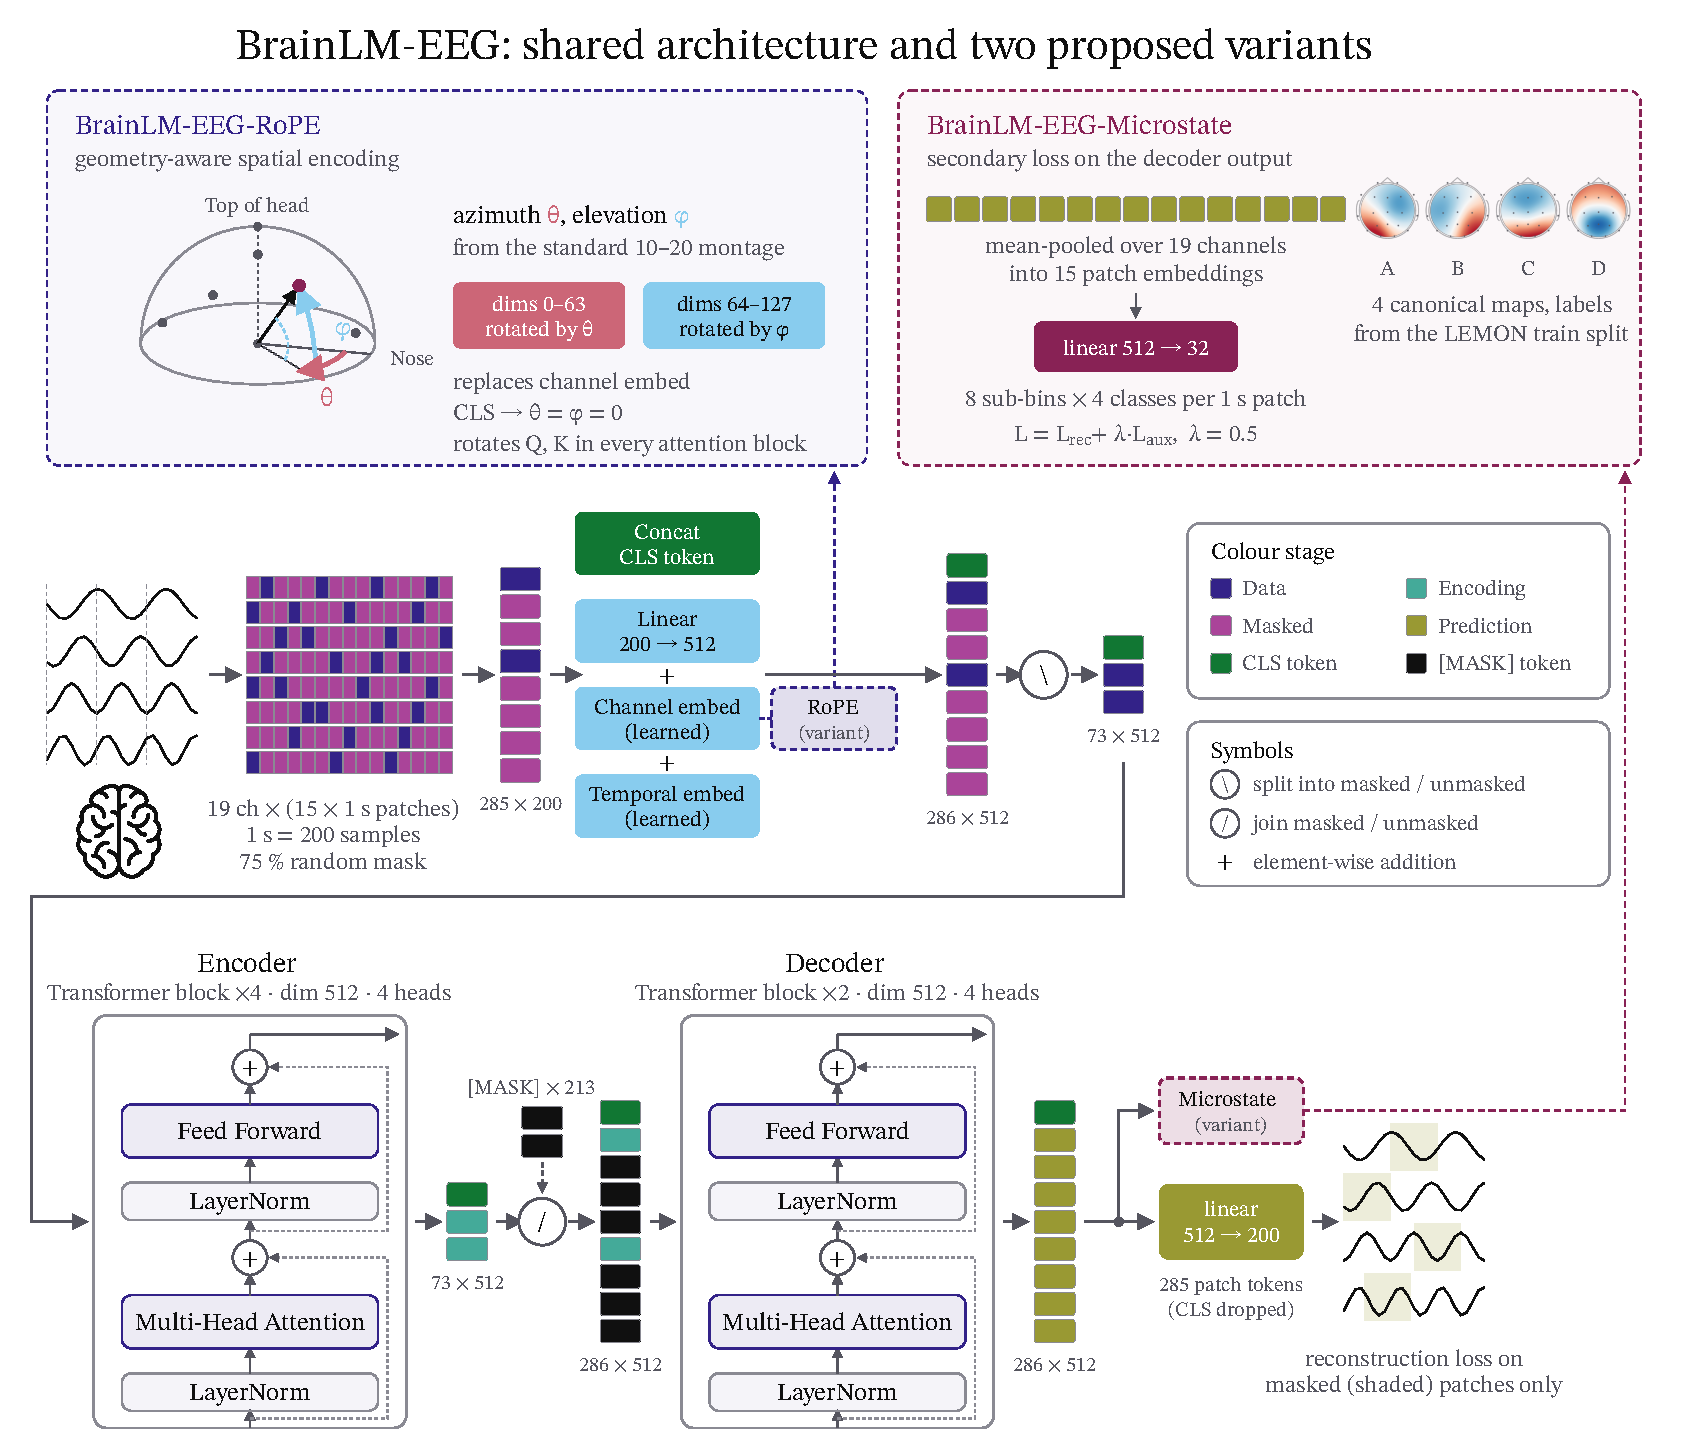
\includegraphics[width=\textwidth]{figures/brainlm-eeg-architecture.pdf}
\caption[Overview of the BrainLM-EEG architecture and variants]{
Overview of the shared BrainLM-EEG architecture and its two variants. 
The backbone performs masked reconstruction of multichannel EEG using channel-time 
patch embeddings, a transformer encoder-decoder, and a linear reconstruction head. 
BrainLM-EEG-RoPE replaces channel embeddings with electrode specific rotary positional 
encoding based on azimuth and elevation. BrainLM-EEG-Microstate adds an auxiliary 
classification head that predicts the microstate class of each 125~ms sub-interval.
}
\label{fig:architecture_overview}
\end{figure}

\subsection{Extensions to BrainLM-EEG}\label{sec:m_proposed_variants}

The two additional variants addressed complementary limitations of the
BrainLM-EEG reference architecture. BrainLM-EEG-RoPE introduced an explicit
representation of relative electrode geometry, whereas
BrainLM-EEG-Microstate incorporated a neurophysiologically informed target into
the self-supervised learning objective. In both variants, all components not
directly related to the proposed modification were kept unchanged. The
comparison with BrainLM-EEG therefore isolates the effect of each extension
from the broader contribution of adapting BrainLM to EEG.

\subsubsection{Geometry-Aware Variant: BrainLM-EEG-RoPE}
\label{sec:m_rope}

Self-attention does not inherently encode token position. In BrainLM-EEG,
spatial position was represented by a learned embedding for each EEG channel.
Although this allowed the model to distinguish electrodes, it did not
explicitly represent the geometric relationships between them. EEG electrodes
are distributed over the approximately spherical surface of the scalp rather
than along a one-dimensional sequence. Each electrode \(c\) was therefore
represented by an azimuth angle \(\theta_c\) and an elevation angle
\(\varphi_c\), obtained from the standard 10-20 montage coordinates. The
coordinate convention, the conversion to these two angles, and their values for
each electrode are given in Appendix~\ref{app:montage}.

BrainLM-EEG-RoPE replaced the learned spatial channel embedding with a rotary
positional encoding based on these electrode coordinates. The learnable
temporal embedding was retained, so the proposed modification affected only
the representation of spatial position.

Rotary positional encoding
\parencite[RoPE;][]{suRoFormerEnhancedTransformer2024} applies position-dependent
rotations to the query and key vectors within self-attention. Consider one
attention head with query vector \(\vq\in\sR^{d}\) and key vector
\(\vk\in\sR^{d}\). Each vector is
partitioned into \(d/2\) consecutive two-dimensional coordinate pairs. For a
token at scalar position \(m\), pair \(i\) is rotated by the angle
\(m\omega_i\), giving the rotation block

\begin{equation}
    \mR_i(m)
    =
    \begin{bmatrix}
        \cos(m\omega_i) & -\sin(m\omega_i) \\
        \sin(m\omega_i) & \phantom{-}\cos(m\omega_i)
    \end{bmatrix},
    \qquad
    \omega_i = b^{-2i/d},
    \qquad
    i = 0,\dots,\frac{d}{2}-1
    \label{eq:rope1d}
\end{equation}

where \(b=10^{4}\). Because rotation matrices satisfy
\(\mR(m)^{\top}\mR(n)=\mR(n-m)\), the attention score between a query at
position \(m\) and a key at position \(n\) can be written as

\begin{equation}
    \bigl(\mR(m)\vq\bigr)^{\top}
    \bigl(\mR(n)\vk\bigr)
    =
    \vq^{\top}\mR(n-m)\vk
    \label{eq:rope_relative}
\end{equation}

The resulting attention score therefore depends on the relative displacement
between positions rather than only on their absolute locations.

Two-dimensional RoPE has previously been used by
\textcite{heoRotaryPositionEmbedding2025} to represent horizontal and vertical
patch coordinates in vision transformers. BrainLM-EEG-RoPE adapted this
principle to EEG electrode geometry. Within each attention head, the first half
of the query and key dimensions were associated with electrode azimuth, while
the second half were associated with electrode elevation. This allocation
yielded \(d/4\) rotation pairs for each coordinate. The rotations were applied
to the query and key vectors in every self-attention layer immediately before
the dot-product attention calculation.

For tokens associated with electrodes \(i\) and \(j\), the resulting attention
score satisfied

\begin{equation}
    \bigl(
        \mR_{2\mathrm{D}}(\theta_i,\varphi_i)\vq
    \bigr)^{\top}
    \bigl(
        \mR_{2\mathrm{D}}(\theta_j,\varphi_j)\vk
    \bigr)
    =
    \vq^{\top}
    \mR_{2\mathrm{D}}
    \bigl(
        \theta_j-\theta_i,
        \varphi_j-\varphi_i
    \bigr)
    \vk
    \label{eq:sphererope}
\end{equation}

Thus, each attention score incorporated the relative azimuthal and elevational
displacement between the corresponding electrodes. The CLS token had
no scalp location and was assigned \(\theta=0\) and \(\varphi=0\). The rotary
encoding was parameter-free with respect to channel identity and depended only
on electrode coordinates, allowing the same mechanism to be applied to
montages or electrode locations not observed during pretraining.

The structure that the rotary encoding imposes on inter-electrode attention, and
the corresponding structure of the learned channel embedding that it replaces,
are shown in Figure~\ref{fig:rope_geometry}.

% Generated by code/analysis/dataset/generate_model_figures.py. Panel (a) calls the
% model's own sphere_rope functions and panel (b) reads the trained spatial_embed
% dumped by analysis/dataset/extract_spatial_embedding.py, so neither can drift
% from the encoder. Authored at \textwidth (6.20 in); do not resize here.
\begin{figure}[htbp]
\centering
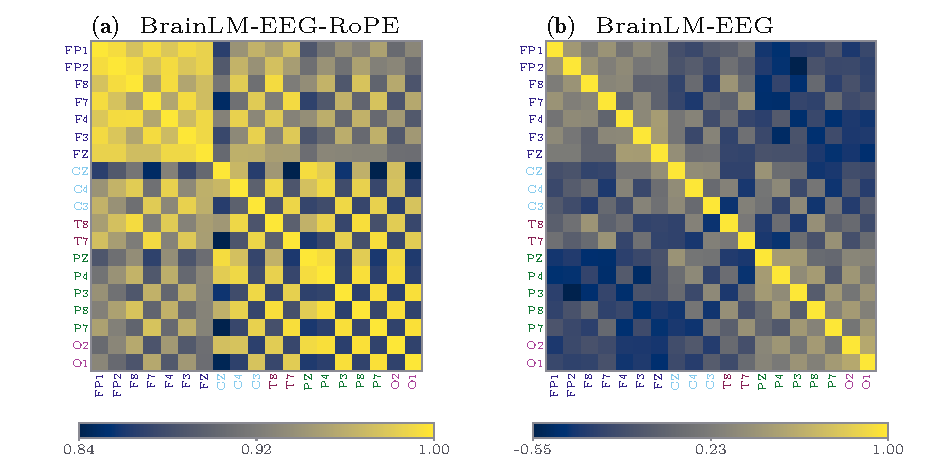
\includegraphics[width=\textwidth]{figures/fig_rope_geometry.pdf}
\caption[Geometry-aware positional encoding]{Comparison of spatial structure in BrainLM-EEG-RoPE and BrainLM-EEG. \textbf{(a)} Expected pairwise attention scores induced by RoPE from the electrode coordinates and fixed throughout training. \textbf{(b)} Pairwise cosine similarity between the channel embeddings learned by BrainLM-EEG after pretraining. Both show spatial organisation across electrodes, but the panels use different quantities and scales and should therefore be compared by pattern rather than magnitude.}
\label{fig:rope_geometry}
\end{figure}

A concurrent positional encoding benchmark by
\textcite{yuceBenchmarkingPositionalEncoding2026} also represented electrode
azimuth and elevation using sinusoidal functions. That approach generated an
absolute positional vector that was added to each token embedding. In
contrast, BrainLM-EEG-RoPE applied a multiplicative rotation within the
attention operation and encoded relative inter-electrode geometry without
altering the token content representation.


\subsubsection{Microstate-Informed Variant: BrainLM-EEG-Microstate}
\label{sec:m_microstate}

BrainLM-EEG was pretrained using masked reconstruction of raw EEG signal
amplitudes. BrainLM-EEG-Microstate extended this objective with an auxiliary
prediction task intended to encourage the model to retain information about
neurophysiologically meaningful resting-state scalp topographies. The
auxiliary objective was added without changing the BrainLM-EEG
encoder-decoder architecture or masking procedure.

During resting-state EEG, the spatial distribution of scalp potentials remains
approximately stable for brief intervals, typically around 80-120~ms, before
transitioning to another configuration. These quasi-stable topographies are
referred to as EEG microstates
\parencite{khannaReliabilityRestingStateMicrostate2014a} and are described in
Section~\ref{sec:bg_microstates}. Four canonical
microstate classes, conventionally labelled A, B, C, and D, have been
repeatedly identified in resting-state EEG and account for a substantial
proportion of the global topographic variance. Their temporal characteristics
have also been reported to differ across several neurological and psychiatric
conditions
\parencite{khannaReliabilityRestingStateMicrostate2014a,michelEEGMicrostatesTool2018a}.
These properties motivated the use of microstate information as an additional
learning target during BrainLM-EEG pretraining.

The canonical microstate maps used in this study were estimated once before
self-supervised pretraining and were subsequently held fixed. They were derived
exclusively from the training partition of the LEMON dataset, which formed part
of the pretraining corpus. No participants assigned to downstream evaluation
were used to estimate these maps. The resulting maps are shown in
Figure~\ref{fig:microstate_maps}.

The number of microstate prototypes was fixed to \(K=4\), corresponding to the
four canonical classes A-D. Microstate topographies were clustered using the
polarity-invariant modified \(k\)-means algorithm
\parencite{391164}, implemented with the \texttt{Pycrostates} Python library
\parencite{Férat2022}. The resulting prototypes were matched to the
conventional A-D ordering by comparison with the reference maps reported by
\textcite{michelEEGMicrostatesTool2018a}. The fixed prototype matrix was
denoted by

\begin{equation}
    \mM
    =
    \begin{bmatrix}
        \vm_1 & \vm_2 & \cdots & \vm_K
    \end{bmatrix}
    \in \sR^{C \times K}
    \label{eq:microstate_matrix}
\end{equation}

where \(C=19\) denotes the number of EEG channels, \(K=4\) denotes the number
of microstate classes, and \(\vm_k\in\sR^{C}\) represents the canonical scalp
topography of microstate class \(k\).

To generate the target labels for the auxiliary task, each one-second temporal
patch was divided into \(S=8\) non-overlapping subintervals of 125~ms. At the
sampling frequency of 200~Hz, each subinterval contained 25 time points. Let
\(p\in\{1,\dots,P\}\) index the one-second temporal patches within a
15-second input window, where \(P=15\), and let
\(s\in\{1,\dots,S\}\) index the 125-ms subintervals within temporal patch
\(p\).

For each subinterval, the signal was averaged over its 25 time points across
each of the \(C\) channels, producing a scalp topography
\(\vz_{p,s}\in\sR^{C}\). The observed topography and each canonical
microstate map were mean-centred across channels, yielding
\(\hat{\vz}_{p,s}\) and \(\hat{\vm}_k\), respectively. The target
microstate label was assigned to the canonical map with the highest absolute
spatial correlation:

\begin{equation}
    y_{p,s}
    =
    \argmax_{k\in\{1,\dots,K\}}
    \left|
        \frac{
            \hat{\vz}_{p,s}^{\top}\hat{\vm}_k
        }{
            \norm{\hat{\vz}_{p,s}}
            \norm{\hat{\vm}_k}
        }
    \right|
    \label{eq:microstate_label}
\end{equation}

where \(y_{p,s}\in\{1,\dots,K\}\) denotes the microstate class assigned to
subinterval \(s\) of temporal patch \(p\). The absolute value makes the
assignment polarity-invariant, such that a scalp topography and its
sign-reversed counterpart are treated as belonging to the same microstate
class.

The auxiliary task required the model to predict the microstate class of each
of the \(S=8\) subintervals within every one-second temporal patch.
Predictions were obtained from the decoder representations. For each
15-second input window, the decoder produced a 512-dimensional representation
for each of the \(C\times P=19\times15=285\) channel-time tokens.

For a given temporal patch \(p\), the \(C=19\) decoder representations
corresponding to the same one-second interval were averaged across channels.
This produced a single 512-dimensional representation for that temporal
patch. Averaging across channels was used because a microstate label describes
the spatial configuration of potentials across the scalp at a given time,
rather than the activity of an individual electrode.

A linear prediction head mapped the pooled representation of each temporal
patch to \(S\times K=8\times4=32\) logits. These logits represented eight
separate four-class predictions, one for each 125-ms subinterval. Let
\(\ve_{p,s}\in\sR^{K}\) denote the vector of \(K\) logits predicted for subinterval \(s\) of temporal
patch \(p\). The element \(\ve_{p,s}[k]\) is therefore the logit assigned by
the model to microstate class \(k\), whereas \(y_{p,s}\) is the target class
defined in Equation~\ref{eq:microstate_label}.

The auxiliary loss was the categorical cross-entropy between the predicted
class distribution and the target microstate class, averaged across all
\(P\) temporal patches and all \(S\) subintervals:

\begin{equation}
    \Ls_{\mathrm{aux}}
    =
    -\frac{1}{P S}
    \sum_{p=1}^{P}
    \sum_{s=1}^{S}
    \log
    \frac{
        \exp\bigl(\ve_{p,s}[y_{p,s}]\bigr)
    }{
        \sum_{k=1}^{K}\exp\bigl(\ve_{p,s}[k]\bigr)
    }
    \label{eq:microstate_aux}
\end{equation}

Here, the denominator applies the softmax normalisation across the \(K\)
candidate microstate classes. The numerator contains the exponential of the
logit assigned to the target class \(y_{p,s}\). Thus, for each subinterval,
the loss is the negative logarithm of the probability assigned by the model to
its target microstate class.

The auxiliary microstate loss was computed for all temporal patches, regardless of which channel-time tokens were masked. In contrast, the
reconstruction loss \(\Ls_{\mathrm{rec}}\) remained unchanged and was
calculated only at masked token positions. This differs from masked prediction approaches such as \textcite{baoBEiTBERTPreTraining2022} and \textcite{baevskiData2vecGeneralFramework2022}, where the prediction objective is restricted to masked positions.

Restricting the auxiliary loss to masked positions was not well suited to the
tokenisation and masking scheme used here. Masking was applied independently
to individual channel-time tokens, whereas a microstate label represented the
scalp topography across all channels within a temporal subinterval. At the
75~\% masking ratio, a given one-second temporal patch generally contained a
mixture of masked and visible channel-time tokens. Moreover, the auxiliary
prediction was obtained by pooling decoder representations across all
channels. Consequently, there was no direct one-to-one correspondence between
an individual masked token and a microstate target. The auxiliary loss was
therefore evaluated for all temporal patches, independently of the
reconstruction mask.

The reconstruction and auxiliary objectives were combined as

\begin{equation}
    \Ls
    =
    \Ls_{\mathrm{rec}}
    +
    \lambda\Ls_{\mathrm{aux}},
    \qquad
    \lambda = 0.5
    \label{eq:microstate_loss}
\end{equation}

where \(\lambda\) controls the contribution of the microstate objective
relative to the reconstruction objective and was fixed to \(0.5\) in this
study.

The auxiliary objective encouraged the model to retain information about canonical scalp topographies and their temporal progression alongside the information required for waveform reconstruction. Microstate labels were used only during pretraining, and the auxiliary prediction head was discarded afterwards. The same BrainLM-EEG encoder was then used for downstream evaluation, so any performance differences reflected the pretraining objective rather than differences in model capacity.

\FloatBarrier

\section{Comparison Baselines}\label{sec:m_baselines}

Three complementary groups of comparison baselines were included: classical
machine learning models trained on handcrafted features, supervised deep
neural networks trained directly on raw EEG, and pretrained EEG foundation
models evaluated using linear probing. Together, these baselines provided
comparisons with conventional feature engineering, task specific end to end
representation learning, and transfer learning from existing pretrained EEG
models.

\subsection{Classical Machine Learning Baselines}\label{sec:m_baselines_ml}

The classical baselines used handcrafted EEG features rather than raw
waveforms. Features were extracted separately from each channel of every
15-second window and concatenated into a single feature vector. Four feature
families were included: spectral band power, time-domain statistics,
discrete-wavelet energy, and continuous-wavelet energy. These feature families
followed the approach used in EEGBench
\parencite{kastratiEEGBenchBenchmarkEEG2025a} and are summarised in
Table~\ref{tab:feature_families}.

Spectral features were computed using Welch's method
\parencite{welchUseFastFourier1967}, which estimates the power spectral density
by averaging spectra from overlapping signal segments. Band power was then
calculated within five EEG frequency bands: \(\delta\) (0.5-4~Hz),
\(\theta\) (4-8~Hz), \(\alpha\) (8-13~Hz), \(\beta\)
(13-30~Hz), and \(\gamma\) (30-45~Hz).

The time-domain features comprised the mean, variance, skewness, kurtosis,
root-mean-square amplitude, zero-crossing rate, Hjorth activity, Hjorth
mobility, Hjorth complexity \parencite{hjorthEEGAnalysisBased1970}, line
length, and peak-to-peak amplitude. Discrete-wavelet features consisted of the
energy of the approximation and detail coefficients obtained using a
Daubechies-4 wavelet \parencite{daubechiesOrthonormalBasesCompactly1988}.
Continuous-wavelet features consisted of Morlet-wavelet energy within the same
five EEG frequency bands \parencite{torrencePracticalGuideWavelet1998}.  Where applicable, feature magnitudes were
transformed using \(\log(1+x)\). Each feature was then standardised to zero
mean and unit variance using parameters estimated from the training partition
only.

\begin{table}[t]
    \centering
    \caption[Handcrafted feature families]{Handcrafted feature families used for the classical
    machine learning baselines. Features were extracted separately from each
    channel and subsequently concatenated. Here, \(L\) denotes the number of decomposition levels used for the
discrete-wavelet transform.}
    \label{tab:feature_families}

    \begin{tabularx}{\textwidth}{>{\raggedright\arraybackslash}p{3.2cm} >{\raggedright\arraybackslash}X c}
        \toprule
        \textbf{Feature family} &
        \textbf{Features represented} &
        \textbf{Features/channel} \\
        \midrule

        Spectral band power &
        Welch band power in the \(\delta\), \(\theta\), \(\alpha\),
        \(\beta\), and \(\gamma\) bands &
        5 \\

        Time-domain statistics &
        Amplitude and temporal signal characteristics, including the Hjorth
        parameters &
        11 \\

        Discrete-wavelet energy &
        Energy of the approximation and detail coefficients from a
        Daubechies-4 decomposition &
        \(L+1\) \\

        Continuous-wavelet energy &
        Morlet-wavelet energy in the five EEG frequency bands &
        5 \\

        \bottomrule
    \end{tabularx}
\end{table}



The resulting feature vectors were classified using linear discriminant
analysis (LDA) \parencite{fisherUseMultipleMeasurements1936}, a linear-kernel
support vector machine (SVM) \parencite{cortesSupportVectorNetworks1995}, and
XGBoost \parencite{chenXGBoostScalableTree2016}.




\subsection{Supervised Deep Learning Baselines}\label{sec:m_baselines_dl}

The supervised deep learning baselines were trained end to end on each
downstream dataset. These models received the preprocessed EEG windows directly
as input, with \(\mX\in\sR^{C\times T}\). All architectures were loaded from
the \texttt{Braindecode} library \parencite{aristimunhaBraindecodeToolboxDecoding2026}, randomly initialised, and
trained using early stopping based on validation loss.

To represent different deep learning approaches to EEG modelling, three
architectures were evaluated. EEGNeX
\parencite{chenReliableSignalsDecoding2024} uses a compact convolutional
architecture with dilated and depthwise-separable convolutions. EEGConformer
\parencite{songEEGConformerConvolutional2023a} combines convolutional feature
extraction with a transformer encoder, allowing both local and longer-range
temporal dependencies to be modelled. ATCNet
\parencite{altaheriPhysicsInformedAttentionTemporal2023} combines
convolutional feature extraction, sliding window multi-head self-attention,
and temporal convolutional modules. Together, these architectures provided a
set of supervised baselines with different modelling strategies, against which
the pretrained BrainLM-EEG representations could be compared.


\subsection{Pretrained EEG Foundation Model Baselines}\label{sec:m_baselines_fm}

The final comparison group consisted of publicly available pretrained EEG
foundation models. Three models were evaluated: LaBraM
\parencite{jiangLARGEBRAINMODEL2024}, CBraMod
\parencite{wangCBraModCrissCrossBrain2025a}, and REVE
\parencite{el2026reve}. For each model, the publicly released
pretrained weights were loaded and the representation backbone was frozen. A
linear classification head was then trained on the corresponding downstream
training partition. This linear probing protocol assessed the separability of
the diagnostic classes in each pretrained representation space without
modifying the encoder.

All BrainLM-EEG models and comparison baselines were evaluated using the same
seed-controlled participant level partitions. Preprocessing, training,
validation, and test partitions were held constant wherever permitted by the
input requirements of the respective models. The same downstream metrics and
model selection criteria were used across model families. This design reduced
the extent to which performance differences could be attributed to differences
in participant allocation or evaluation procedure.


% TODO: Combined pretraining corpus (LEMON/SRM/DVS train + clinical pretrain-reserve
% pools). Optimizer AdamW; LR linear-scaling rule (eff_lr = base_lr x batch/256);
% warmup + cosine schedule; up to 500 epochs with early stopping; batch 512; weight
% decay 0.05 on weights only. Explain the BrainLMEEG-1k variant (what "1k" denotes -
% larger/longer pretraining). Mention the online linear probe used to monitor
% representation quality during pretraining.

\FloatBarrier

\section{Self-Supervised Pretraining}\label{sec:m_pretrain}

BrainLM-EEG, BrainLM-EEG-RoPE, and BrainLM-EEG-Microstate were pretrained using the same data partitions and optimisation procedure. The variants differed only in the architectural or objective level modifications described in Section~\ref{sec:m_proposed_variants}. The remaining pretraining settings were kept fixed to support a direct comparison between the model variants.

The pretraining corpus comprised resting-state EEG data from six datasets, allocated as described in Section~\ref{sec:m_datasets}: the training partitions of DVS, SRM, and LEMON, together with the pretraining reserve subsets of ADFTD, FEP, and MDD. Because the clinical reserve subsets were comparatively small, they were used entirely for pretraining and were not divided further.

The resulting corpus and its demographic composition are shown in
Figure~\ref{fig:pretrain_cohorts}. The three
healthy control datasets contribute the large majority of the participants,
while the clinical reserve subsets contribute the diagnostic and age variability
that those datasets lack.

All models used the common set of 19 EEG channels described in Section~\ref{sec:m_brainlmeeg}. Recordings were divided into non-overlapping 15-second windows sampled at 200~Hz, giving inputs of \(\mX \in \sR^{19 \times 3000}\). Per-window, per-channel \(z\)-score normalisation was applied during data loading as described in Section~\ref{sec:m_preprocess}. The normalised windows were then processed using the spatiotemporal patching, tokenisation, masking, and reconstruction procedures described in Section~\ref{sec:m_brainlmeeg}.

% Generated by code/analysis/dataset/generate_results_figures.py, which writes
% the PDF directly into manuscript/figures/. Authored at \textwidth (6.20 in)
% so the include applies no scaling. Do not resize here.
\begin{figure}[htbp]
\centering
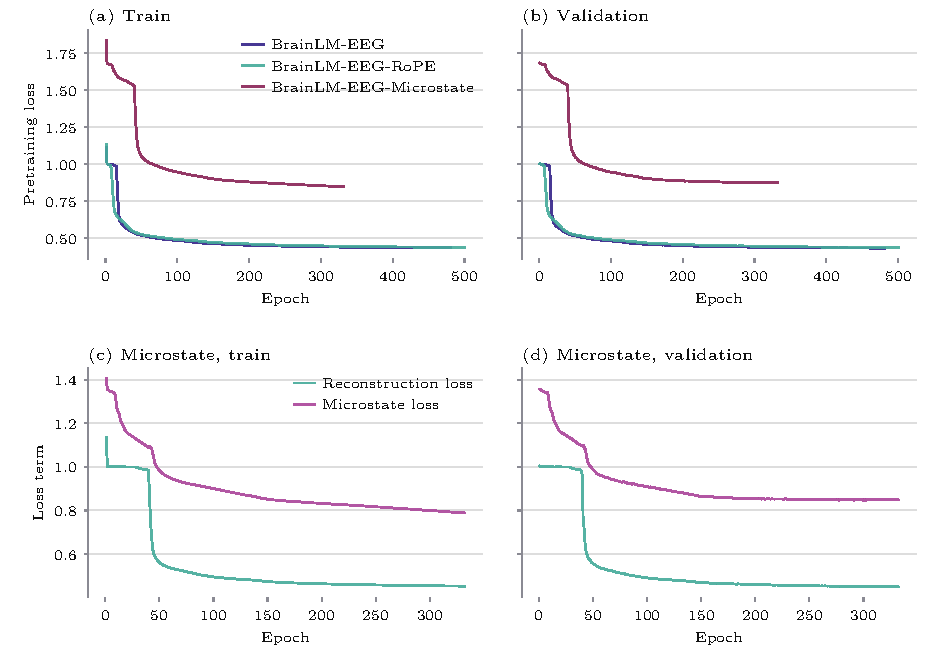
\includegraphics[width=\textwidth]{figures/fig_pretrain_curves.pdf}
\caption[Pretraining loss trajectories]{
Pretraining loss trajectories for the three model variants; lines end at each
variant's early-stopped epoch. \textbf{(a,b)} Train and validation total loss.
For BrainLM-EEG and BrainLM-EEG-RoPE, this is the reconstruction loss
\(\Ls_{\mathrm{rec}}\); for BrainLM-EEG-Microstate, it is the combined objective
\(\Ls=\Ls_{\mathrm{rec}}+0.5\Ls_{\mathrm{aux}}\) from Equation~\ref{eq:microstate_loss}.
\textbf{(c,d)} Separate reconstruction and microstate losses for
BrainLM-EEG-Microstate. Panels within each row share a vertical scale.
}
\label{fig:pretrain_curves}
\end{figure}

All models were optimised using AdamW \parencite{loshchilovDecoupledWeightDecay2019} with a batch size of 512. The learning rate was set using the linear scaling rule \parencite{goyalAccurateLargeMinibatch2018}, with a base learning rate of \(1.5\times10^{-4}\) defined for a batch size of 256. For the batch size of 512 used here, this resulted in a learning rate of \(3\times10^{-4}\). A weight decay of \(0.05\) was applied to weight parameters, while bias and normalisation parameters were excluded from weight decay. The learning rate increased linearly from zero during the first 40 epochs and subsequently decreased towards zero using cosine decay. Gradients were clipped to a maximum global norm of \(1.0\).

Models were pretrained for a maximum of 500 epochs. Early stopping was applied when the validation reconstruction loss did not improve for 30 consecutive epochs, and the checkpoint with the lowest validation reconstruction loss was retained for downstream evaluation. Using the same reconstruction-based stopping and checkpoint-selection criterion for all variants kept the model selection procedure consistent across the comparison.

A diagnostic linear probe was performed every 50 epochs to monitor the development of the learned representations. At each interval, the encoder was frozen and a linear classification head was trained on the Alzheimer's disease versus healthy control task using the same participant level partitions as the corresponding downstream evaluation. The probe was used only as a training diagnostic; its performance did not affect encoder optimisation, early stopping, or checkpoint selection and was therefore not included in the reported downstream results. The pretraining loss trajectories are shown in Figure~\ref{fig:pretrain_curves}.


\section{Downstream Evaluation}\label{sec:m_protocols}

The downstream evaluation assessed whether the representations learned during self-supervised pretraining transferred to diagnostic classification tasks. Four binary classification tasks were considered: Alzheimer's disease (AD) versus healthy controls, frontotemporal dementia (FTD) versus healthy controls, first-episode psychosis (FEP) versus healthy controls, and major depressive disorder (MDD) versus healthy controls.

\subsection{Subject Level Prediction and Evaluation Metrics}\label{sec:m_metrics}

All downstream performance was evaluated at the participant level because multiple EEG windows from the same participant are not independent observations. Let \(p_{s,i}\) denote the predicted probability of the patient class for window \(i\) from participant \(s\), and let \(N_s\) denote the number of windows from that participant. The continuous participant level score was calculated as the mean patient class probability across windows,

\begin{equation}
\bar{p}_s =
\frac{1}{N_s}
\sum_{i=1}^{N_s} p_{s,i}.
\label{eq:subject_probability}
\end{equation}

For metrics requiring a hard class prediction, each window was assigned to the class with the higher predicted probability, and the participant level prediction was obtained by majority vote across its windows. In the case of an equal vote, the tie was resolved using the mean patient class probability \(\bar{p}_s\).

Balanced accuracy (BAcc) and area under the precision-recall curve (AUPRC) were used as the primary evaluation metrics. Balanced accuracy was used because the downstream datasets were not perfectly class balanced, with the largest imbalance occurring in MDD. It gives equal weight to sensitivity and specificity and was calculated as

\begin{equation}
\mathrm{BAcc}
=
\frac{1}{2}
\left(
\frac{\mathrm{TP}}{\mathrm{TP}+\mathrm{FN}}
+
\frac{\mathrm{TN}}{\mathrm{TN}+\mathrm{FP}}
\right).
\label{eq:balanced_accuracy}
\end{equation}

where \(\mathrm{TP}\), \(\mathrm{TN}\), \(\mathrm{FP}\), and \(\mathrm{FN}\) denote the numbers of true positives, true negatives, false positives, and false negatives, respectively, with the patient group treated as the positive class. 


AUPRC was computed using the average-precision formulation, with the patient group treated as the positive class. The participant level probability \(\bar{p}_s\) was used as the continuous score for this calculation. Balanced accuracy therefore used the majority vote participant label, whereas AUPRC used the mean patient class probability across windows.

% TODO: Check for spelling grammar and rewrite

AUPRC was preferred to the area under the receiver operating characteristic curve (AUROC) because the clinical objective was not only to separate patients from healthy controls, but also to ensure that participants identified as having a disorder were likely to have it. AUPRC is more informative under class imbalance and is the more clinically relevant summary for this question. The average precision of the patient class alone was reported, rather than the mean of the patient and healthy class values, because averaging the two would have returned the chance level to 0.5 for every task and hidden exactly the sensitivity to class imbalance that motivated the choice of AUPRC.


\subsection{Linear Probing and Finetuning}\label{sec:m_lp_ft}

Two adaptation settings were evaluated. For linear probing, the pretrained encoder was frozen and a three-layer classification head was trained using the CLS token representation. This setting evaluated how informative the pretrained representation was for each downstream task without modifying the encoder.

For finetuning, both the pretrained encoder and the classification head were updated using the downstream training data. A learning rate of \(5\times10^{-5}\) was used to allow task specific adaptation while limiting the magnitude of updates to the pretrained encoder. Comparing linear probing and finetuning provided complementary measures of how well the pretrained representations transferred to the downstream tasks.

The same classification head was used in both settings, so they differ only in whether the encoder was updated. The architecture of the head and the complete optimisation settings for both are given in Appendix~\ref{app:adaptation}.


\subsection{Within-Dataset Cross-Validation}\label{sec:m_fivefold}

Because the downstream datasets contained relatively few participants, within-dataset evaluation was performed using five-fold cross-validation. The folds were constructed at the participant level using a fixed random seed and were stratified by diagnostic class. All windows from a participant were assigned to the same fold to prevent participant level leakage between training, validation, and test sets.

For each run, three folds were used for training, one for validation, and one for testing. The fold assignments were rotated across five runs so that each fold served as the test set once. This produced five trained models for each task and adaptation setting. Performance was evaluated on the held-out test participants and averaged across the five runs. This evaluation measured generalisation to unseen participants from the same dataset. The fold structure is illustrated in Figure~\ref{fig:eval_protocol_fivefold}.

\begin{figure}[htbp]
\centering
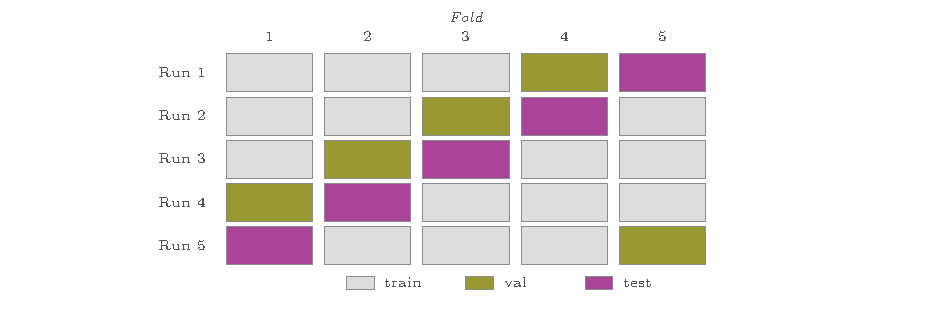
\includegraphics[width=\textwidth]{figures/fig_eval_protocol_rolling.pdf}
\caption[Five-fold cross-validation]{Five-fold participant level
cross-validation. Fold assignment for each of the five cross-validation runs.}
\label{fig:eval_protocol_fivefold}
\end{figure}


\subsection{Leave-One-Subject-Out Evaluation}\label{sec:m_loso}

The five-fold experiments showed relatively large variation across folds for some tasks. A leave-one-subject-out (LOSO) evaluation was therefore additionally performed to reduce dependence on a particular five-fold partition and to obtain an out-of-sample prediction for each participant.

For a dataset containing \(N\) participants, each LOSO iteration used one participant as the test subject, one different participant as the validation subject, and the remaining \(N-2\) participants for training. Training continued according to the early-stopping criterion, and the checkpoint with the lowest validation loss was selected. The selected checkpoint was then evaluated on the held-out test participant. This procedure was repeated until every participant had served as the test subject once. The resulting subject level predictions were pooled to calculate the final performance metrics. The procedure is illustrated in Figure~\ref{fig:eval_protocol_loso}.

\begin{figure}[htbp]
\centering
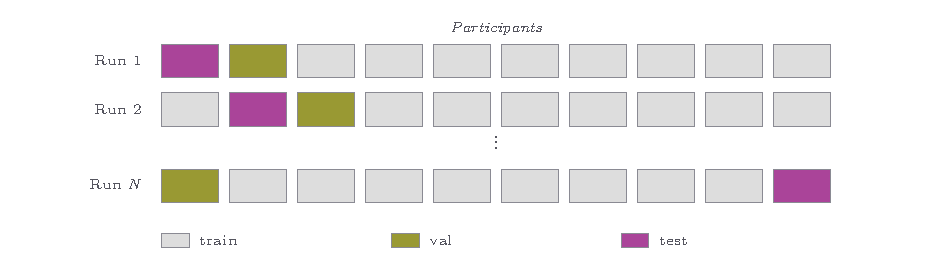
\includegraphics[width=\textwidth]{figures/fig_eval_protocol_loso.pdf}
\caption[Leave-one-subject-out cross-validation]{Leave-one-subject-out
cross-validation. Participant assignment for three representative runs;
the ellipsis marks the remaining runs up to run \(N\).}
\label{fig:eval_protocol_loso}
\end{figure}


\subsection{Cross-Dataset Evaluation}\label{sec:m_crossdataset}

Cross-dataset evaluation was used to examine transfer to data collected in a different dataset. The five models trained on the FEP dataset during cross-validation were each evaluated on the independent SCZ dataset, and their performance was averaged. In addition, a model trained using the full FEP development data was evaluated on SCZ. This provided an external evaluation of how well representations learned from FEP data transferred to a separate schizophrenia dataset. This transfer setting is illustrated in Figure~\ref{fig:eval_protocol_crossdataset}.

\begin{figure}[htbp]
\centering

\includegraphics[width=\textwidth]{figures/fig_eval_protocol_crossdataset.pdf}
\caption[Cross-dataset transfer]{Cross-dataset transfer. Models trained on
FEP (\(n=62\)) are evaluated on the independently acquired SCZ cohort
(\(n=77\)).}
\label{fig:eval_protocol_crossdataset}
\end{figure}


\FloatBarrier

\section{Ablation Studies and Model Analysis}\label{sec:m_probes}
% \subsection{Masking Strategy Ablation}\label{sec:m_masking}
% TODO: The strategies compared: random {20,50,75,90}%, channel-wise, temporal
% (causal / random), brain region. Neuroscience analogy for each. 75% random is the
% canonical baseline.
% \subsection{Layer-Wise Representation Probing}\label{sec:m_layerprobe}
% TODO: Probe each encoder layer individually + aggregations (final, weighted sum),
% to locate where the most class-discriminative representation lives.
% \subsection{CLS-Token Information Test}\label{sec:m_clstest}
% TODO: Motivate the concern (the reconstruction loss never directly supervises the
% CLS token). Protocol: encode once; decode with original versus corrupted CLS token
% (zeros / Gaussian noise) on held-out data; Wilcoxon signed-rank test on paired
% per-batch reconstruction losses. Significant increase => CLS is load-bearing.
% \subsection{Reconstruction-as-Features Analysis}\label{sec:m_reconfeat}
% TODO: Encode->decode the signal (mask_ratio = 0, full autoencoder) and classify the
% RECONSTRUCTED signal versus the RAW signal with a fixed downstream model, testing
% whether the learned manifold preserves/enhances class-discriminative structure.



In addition to the downstream evaluation, a set of ablation and analysis experiments was conducted to examine how selected modelling choices affected model behaviour and downstream performance. These experiments considered the masking configuration used during pretraining, the information available at different encoder layers, the contribution of the CLS token to reconstruction, and the extent to which reconstructed EEG retained information relevant to downstream classification.

\subsection{Masking Strategy and Masking Ratio}\label{sec:m_masking_ablation}

% Generated by code/analysis/dataset/generate_ablation_figures.py, which writes
% the PDFs directly into manuscript/figures/. Authored at \textwidth (6.20 in)
% so the include applies no scaling. Do not resize here.
\begin{figure}[htbp]
\centering
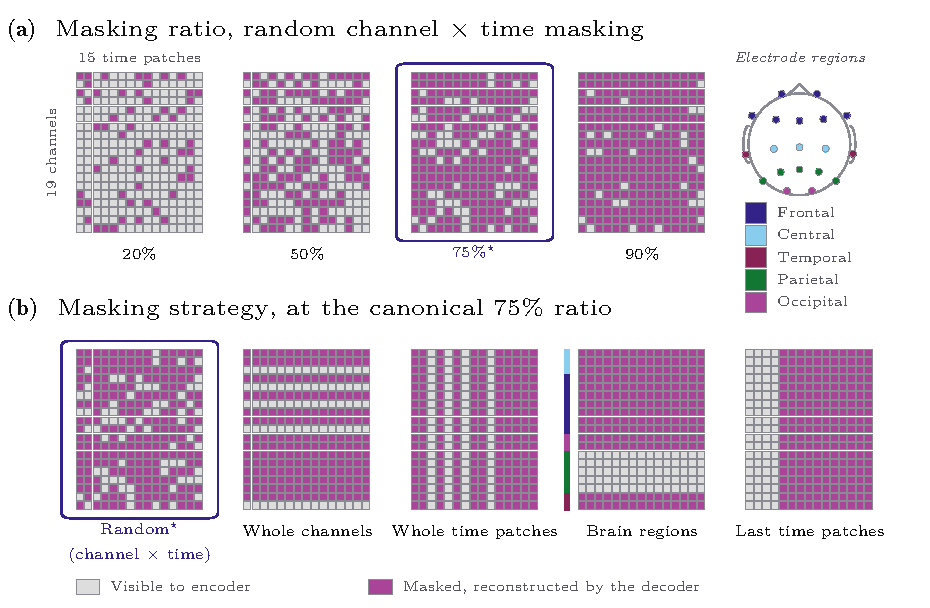
\includegraphics[width=\textwidth]{figures/fig_masking_schemes.pdf}
\caption[Masking ratios and masking strategies]{The nine pretraining masking
variants, drawn on the \(19 \times 15\) grid of spatiotemporal tokens produced
by a single 15-second window: rows are the 19 channels in the order the model
receives them, columns are the 15 one-second temporal patches, and shaded cells
are the tokens withheld from the encoder and reconstructed by the decoder.
Starred panels mark the canonical setting used for BrainLM-EEG elsewhere in
this work. Each pattern is one representative random draw under a fixed seed.
In the brain region panel, whole regions are masked at random until the
closest total under the nominal ratio is reached; the colour bar at that
panel's left edge marks the region blocks and is keyed to the scalp map
in~\textbf{(a)}.}
\label{fig:masking_schemes}
\end{figure}

The baseline BrainLM-EEG configuration described in Section~\ref{sec:m_brainlmeeg} used a masking ratio of 75\% with random spatiotemporal masking. To examine the effect of the amount of masked input, additional models were pretrained using masking ratios of 20\%, 50\%, and 90\%, while the remaining pretraining settings were kept unchanged.

The masking structure was also varied to examine whether different forms of missing information affected representation learning. The evaluated strategies included masking complete channels across time, masking randomly selected temporal regions across all channels, masking the final portion of the input window across all channels, and region-wise masking in which electrodes were grouped by anatomical brain region and all electrodes within a selected region were masked together. These strategies were intended to represent different forms of missing spatial or temporal information, including missing electrodes and forecasting-like reconstruction. All variants were evaluated using the downstream protocol described in Section~\ref{sec:m_protocols}. The nine resulting variants are shown in Figure~\ref{fig:masking_schemes}.




\subsection{Layer-Wise Representation Analysis}\label{sec:m_layer_probe}

\begin{figure}[htbp]
\centering
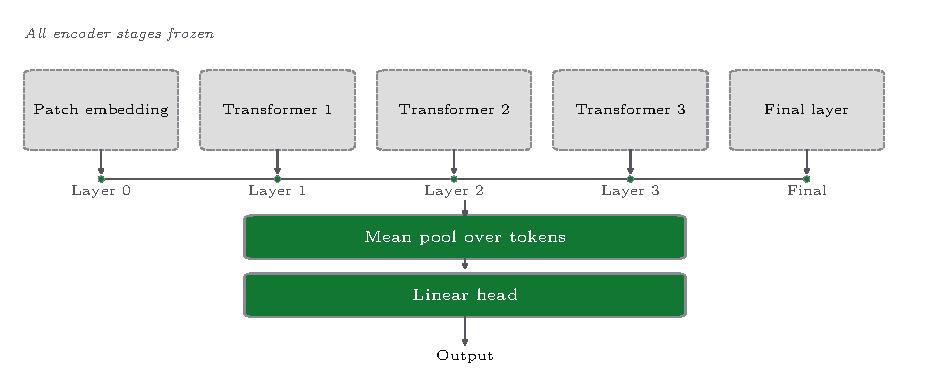
\includegraphics[width=\textwidth]{figures/fig_layer_probe.pdf}
\caption[Layer-wise probing]{Layer-wise probing of the pretrained BrainLM-EEG encoder with frozen encoder weights. A separate linear head is trained on token-averaged representations from each encoder stage; layer 0 denotes the patch embedding.}
\label{fig:layer_probe}
\end{figure}


A layer-wise probing experiment was performed to examine how task relevant information was distributed across the encoder. After pretraining, the encoder was frozen and representations were extracted from each encoder stage. For each stage, the token representations were averaged across the sequence to obtain a single representation for each EEG window. A separate linear classification head was then trained on the resulting representation.

Each encoder stage was evaluated separately using the same downstream evaluation protocol described in Section~\ref{sec:m_protocols}. This analysis was used to compare the amount of downstream discriminative information available at different depths of the encoder and to determine how this information emerges and evolves throughout the learned representation hierarchy. The overall probing procedure is illustrated in Figure~\ref{fig:layer_probe}.


\subsection{CLS Token Contribution to Reconstruction}\label{sec:m_cls_analysis}

BrainLM-EEG uses a masked autoencoder architecture in which the encoder maps an EEG window to latent token representations, including a CLS token, and the decoder reconstructs the masked input from these representations. Although the CLS token is used for downstream classification, it is not directly supervised by a classification objective during self-supervised pretraining. An additional analysis was therefore performed to examine whether the decoder made use of the CLS representation during reconstruction.

EEG windows from the pretraining validation set were first passed through the pretrained encoder. Reconstruction was then performed under three conditions: (1) using the encoder output without modification, (2) replacing the CLS representation with zeros, and (3) replacing the CLS representation with Gaussian noise. All other latent token representations were left unchanged. Reconstruction error was measured using the same mean squared error objective used during pretraining.

Because the same EEG windows were evaluated under each condition, paired Wilcoxon signed-rank tests were used to compare the reconstruction losses obtained with the unmodified CLS token and the perturbed CLS conditions. An increase in reconstruction error after perturbing the CLS token would indicate that information carried by this token contributes to the decoder's reconstruction. This procedure is summarised in Figure~\ref{fig:cls_test}.

\begin{figure}[htbp]
\centering
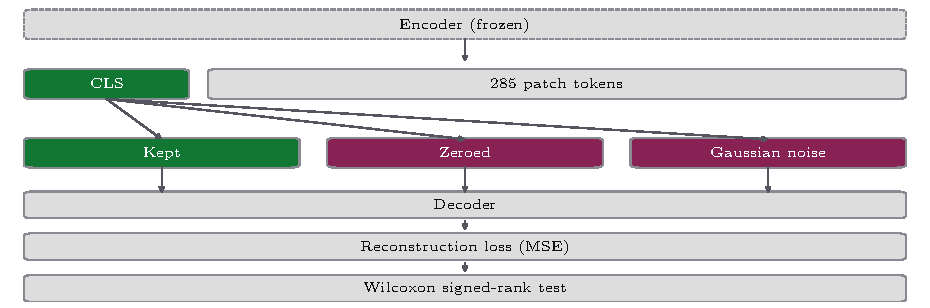
\includegraphics[width=\textwidth]{figures/fig_cls_test.pdf}
\caption[CLS token test]{CLS token test on the pretrained BrainLM-EEG encoder with frozen encoder weights. Each window is encoded once, and reconstruction is evaluated with the CLS latent kept, zeroed, or replaced by Gaussian noise. Paired losses are compared using a Wilcoxon signed-rank test; increased loss under corruption indicates CLS-token use.}
\label{fig:cls_test}
\end{figure}


\subsection{Analysis of Reconstructed EEG}\label{sec:m_reconstruction_analysis}

A final experiment examined whether EEG reconstructed by the pretrained encoder-decoder retained information relevant to downstream classification. EEG windows from the downstream datasets were passed through the pretrained model to obtain reconstructed signals. The same baseline classifiers used elsewhere in the study, including LDA and ATCNet, were then trained separately using either the original EEG windows or the corresponding reconstructed windows.

The models were evaluated using the same participant level downstream protocol described in Section~\ref{sec:m_protocols}, and performance obtained from original and reconstructed EEG was compared. This analysis assessed the extent to which the reconstructed signals retained information used by the downstream classifiers to distinguish patients from healthy controls. Figure~\ref{fig:reconstruction_features} summarises this comparison.

\begin{figure}[htbp]
\centering
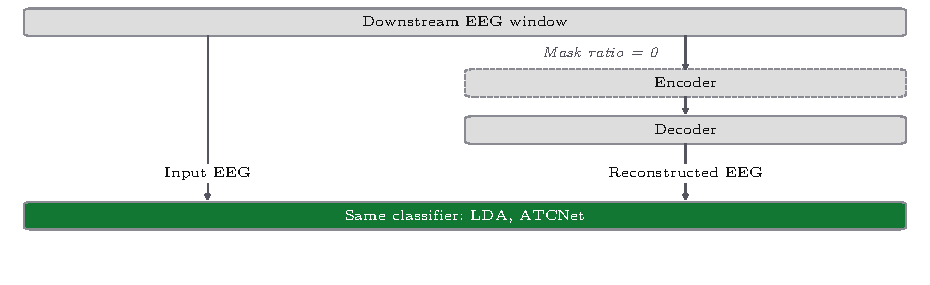
\includegraphics[width=\textwidth]{figures/fig_reconstruction_features.pdf}
\caption[Reconstruction as features]{Reconstruction as features using the pretrained BrainLM-EEG encoder-decoder with frozen weights. The same classifier is trained on the original and reconstructed windows (masking ratio \(=0\)) to assess whether class discriminative information is preserved.}
\label{fig:reconstruction_features}
\end{figure}

\FloatBarrier
